\section{RationalGRL: Logical Framework}
\label{sect:formalframework}

In Section~\ref{sect:gmas} we developed a list of critical questions and argument schemes by analyzing transcripts of discussions about the development of a traffic simulator. The resulting list is shown in Table~\ref{table:argument-schemes}. We then presented the RationalGRL framework in secton~\ref{sect:overview}, consisting of a modeling language, a metamodel, and various examples of using the argument schemes and critical questions. In section~\ref{sect:meth+tool} we explained how this framework can be used by practitioners by explaining the methodology and tool support.

In this section we present a formalization of RationalGRL based on formal logic. This is done for multiple reasons: (i) Most approaches in formal argumentation use formal logic, allowing us to employ existing technique directly in order to compute which arguments are accepted and which are rejected, (ii) we can be more precise about how critical questions are answered, (iii) we can show that RationalGRL models can be translated in to valid GRL models and visa versa in a precise way, and (iv) the formal approach is a basis for automating the framework in terms of tool support.

In the first two subsections we formalize a static representation of our framework: We provide a formal specification of a GRL model based on the GRL metamodel (Section \ref{sect:metamodel}) in the first subsection, and we extend this with arguments and attack links in the second subsection, hereby obtaining a formal specification of a RationalGRL model. 

In the third subsection we develop algorithms in order to translate a GRL model into a RationalGRL model, and visa versa.

In the fourth and final subsection we turn to the dynamics of our framework. We develop algorithms for instantiating argument schemes and for answering critical questions. 

\subsection{Formal Specification of GRL}
\label{sect:formalframework:grl}

In this subsection we formalize a GRL model based on the GRL metamodel and the jUCMNav implementation. We first formalize elements of GRL (intentional elements and actors), and then formalize the links.

\subsubsection{Intentional Element, beliefs and actors}

We start with some general definition that we use in subsequent definitions.

\begin{definition}[General definitions]
\label{def:set-definitions}
Throughout this section, we adopt the convention that variables start with a lowercase letter (e.g, $id, i, j, name, ie, goal$), and sets and constants start with an uppercase letter (e.g., $Type, AND, Goal$).

We define the following sets:
\begin{itemize}
\item $IETypes = \{Softgoal, Goal, Task, Resource\}$,
\item $LinkTypes = \{PosContr, NegContr, Dep, Decomp\}$\footnote{Note that for decomposition links, we only distinguish between a positive contribution ($PosContr$) and a negative contribution ($NegContr$). The GRL metamodel specifies a total of seven contribution values. We instead have chosen only two here to simplify some of the notation, but it is straightforward to extend this to seven values.},
\item $Types = IETypes \cup LinkTypes\cup\{Actor, GenArg, ActIE\}$,
\item $Names$ is a finite set of strings,
\item $DecompTypes = \{AND,OR,XOR\}$.
\end{itemize}
\end{definition}

Next we define an intentional element.

\begin{definition}[Intentional Element]
\label{def:ie}
An intentional element $ie\in \mathbb{N}\times IETypes\times Names\times DecompType$ is a tuple, where $ie = (id, type, name, decomptype)$ means:
\begin{itemize}
\item $id\in \mathbb{N}$ is a unique identifier for the element,
\item $type\in IETypes$ specifies the type of the element,
\item $name \in Names$ is a string description of the element,
\item $decomptype\in DecompType$ refers to the type of decomposition.\footnote{Note that the decomposition type is relevant only if the element is in fact decomposed into other elements, but since the jUCMNav implementation defines the decomposition type on the element, we do the same here.}
\end{itemize}
A set of intentional elements is denoted by $IE$.
\end{definition}

The definition above is sufficient to capture all intentional elements used in GRL. However, we present some syntactic sugar in the next definition by abbreviating the definition above in various ways. This does not add anything new to the previous definition, but it simplifies some of the notation.

\begin{definition}[Notation]
\label{def:notation}
We adopt three conventions simplifying our notation:
\begin{itemize}
\item
We refer to the element of a tuple using the dot (".") notation. That is, we may for instance refer to the id, type, name and decomposition type of an $IE$ with respectively $ie.id$, $ie.type$, $ie.name$, and $ie.decomptype$.
\item 
We refer to a set of elements with the same id $i$  using the $i$ subscript on the set. For instance a set of IEs with id $i$ is denoted by $IE_i$, and if this is a single element, we denote it by $ie_i$\footnote{In GRL, there always exists at most one element for every id (see Def.~\ref{def:grl-model}), in RationalGRL, however, this condition does not hold (see Def.~\ref{def:rationalgrl-model}).} For instance, we may refer to the intentional element $ie = (0, Goal, \text{Make profit}, AND)$ with $ie_0$ and write $ie_0.type = Goal$, $ie_0.name = \text{Make profit}$, and $ie_0.decompositiontype = AND$. 
\item
We can also refer to intention elements of a specific type simply by $type_{id}$. For instance, we can abbreviate the element in the previous item with $goal_0$ and write $goal_0.name = \text{Make profit}$, and $goal_0.decomptype = AND$.
\end{itemize}
\end{definition}

\paragraph{Rationale and example} Throughout this section we use the example in Figure~\ref{fig:example-small}, which is shown in Figure~\ref{fig:example-small2} as well. Our formalization of GRL is very much in line with the way in which GRL models are represented in the open-source Eclipse-based tool jUCMNav.\footnote{See \url{http://jucmnav.softwareengineering.ca/foswiki/ProjetSEG}} This tool is actively developed and has a rich number of features for the analysis of both GRL and URN models. By keeping our formalization in line with this tool, we simplify the translation step from models in the RationalGRL tool to models in the jUCMNav tool.

Some of the IEs in Figure~\ref{fig:example-small2} can be formalized using Def.~\ref{def:ie} as follows:
\begin{itemize}
\item $(4, Goal, \text{Generate traffic}, XOR)$: This represents the goal ``Generate traffic'', which is XOR-decomposed. Note the identifier ``2'' is not shown in the GRL model, but it is stored internally.
\item $(1, Resource, \text{Car objects}, AND)$: Although this element does not decompose into any other elements, it still contains an AND-decomposition. Our motivation for this choice is that it simplifies the formalization of decomposition links. It is in line with with GRL metamodel and the jUCMNav implementation.
\end{itemize}

Using the short-hand notation defined in Def.~\ref{def:notation}, we can make the following statements:
\begin{itemize}
\item $goal_4.name = \text{Generate traffic}$
\item $goal_4.decomptype = XOR$
\item $resource_1.name = \text{Car objects}$
\end{itemize}

\begin{figure}[ht]
\centering
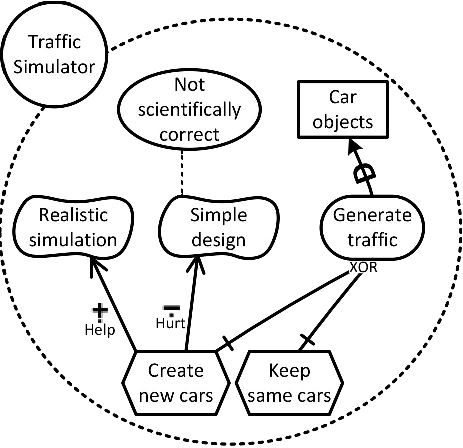
\includegraphics[width=\columnwidth]{img/Example1-new.pdf}
\caption{Example GRL model (reprint of Fig.~\ref{fig:example-small})}
\label{fig:example-small2}
\end{figure} 

\begin{definition}[Actor]
\label{def:actor}
An actor $act \in \mathbb{N}\times {Actor}\times Names$ is a tuple where $act=(id,Actor, name)$ means:
\begin{itemize}
\item $id\in\mathbb{N}$ is the identifier of the actor, 
\item $Actor$ states that this tuple is an actor,\footnote{While this element may look redundant in this tuple, it will become important when translating between RationalGRL models and GRL models. Otherwise it would not be possible to identify this tuple as an actor.}
\item $name\in Names$ is a string description of its name.
\end{itemize}

Similar to intentional elements, we may refer to $act = (id,name)$ with $act_{id}$ and write $act_{id}.name$ to refer to its name.

A set of actors is denoted by $Act$.
\end{definition}

\paragraph{Rationale and example} An actor is simply a pair consisting of its identifier and its name. The relation between actors and their intentional element is formalized in the next definition. 

We can formalize the actor of Figure~\ref{fig:example-small2} as $act=(0,Actor,\text{Traffic Simulator})$, and we can for instance state $act_0.name = \text{Traffic Simulator}$.

\begin{definition}[Actor-IE Relations]
\label{def:act-ie-relation}
An \emph{Actor-IE relation} $r_{ActIE}\in\mathbb{N}\times\{ActIE\}\times\mathbb{N}\times\mathbb{N}$ is a tuple where $r_{ActIE}=(id,ActIE, i, j)$ means:
\begin{itemize}
\item $id\in\mathbb{N}$ is the identifier of the relation, 
\item $ActIE$ states that this tuple is an Actor-IE relation,
\item $i\in\mathbb{N}$ is an id of an actor,
\item $j\in\mathbb{N}$ is an id of an IE.
\end{itemize}

A set of Actor-IE relations is denoted by $R_{ActIE}$.
\end{definition}

\paragraph{Rationale and example} The previous definition specifies relations between actors and intentional elements. Each actor can own one or multiple intentional elements, but each intentional element can only be owned by at most one actor (we will make these assumptions explicit in Def.~\ref{def:valid-grl-model}).

In Figure~\ref{fig:example-small2}, recall we formalized two IEs and the actor as follows:
\begin{itemize}
\item $(1, Resource, \text{Car objects}, AND)$
\item $(4, Goal, \text{Generate traffic}, XOR)$
\item $(0, \text{Traffic Simulator})$
\end{itemize}

We can then formalize the Actor-IE relationships for these elements as:
\begin{itemize}
\item $(12, ActIE, 0, 1)$
\item $(15, ActIE, 0, 4)$
\end{itemize}

\subsubsection{Links}

At this point we have defined all intentional elements in GRL and a containment relation between actors and intentional elements. We now turn to the GRL links.

\begin{definition}[GRL Link]
\label{def:link}
A \emph{GRL link}: $link\in \mathbb{N}\times LinkTypes\times \mathbb{N}\times\mathbb{N}$ is a tuple such that $link = (id,type,src,dest)$ means
\begin{itemize}
\item $id\in \mathbb{N}$ is the unique identifier of the link,
\item $type\in LinkTypes$ specifies the type of the link, 
\item $src\in \mathbb{N}$ is the identifier of the IE from which the link starts,
\item $dest\in \mathbb{N}$ is the identifier of the IE at which the link ends.
\end{itemize}

A set of links is denoted by $Link$.
\end{definition}

We also introduce some simplified notation for the links.

\begin{definition}[Notation]
\label{def:notation2}
\begin{itemize}
\item
We can refer to links of a specific type simply by $type_{id}$. For instance, we can abbreviate the link $(0,PosContr,2,3)$ with $posContr_0$. 
\item 
We can refer to a set of positive contribution links, negative contribution links, dependency links, and decomposition link with respectively $PosContr, NegContr, Dep,$, and $Decomp$. 
\item
We can refer to a set of contribution links that can be either positive or negative simply with $Contr$.
\end{itemize}
\end{definition}

\paragraph{Rationale and example} Similar to IEs, links have identifiers as well. In Fig.~\ref{fig:example-small2}, there are five links. First, let us formalize the related IEs:
\begin{itemize}
\item (1, Resource, \text{Car objects}, AND),
\item (2, Softgoal, \text{Realistic simulation}, AND),
\item (3, Softgoal, \text{Simple design}, AND),
\item (4, Goal, \text{Generate traffic}, XOR),
\item (5, Task, \text{Create new cars}, AND),
\item (6, Task, \text{Keep same cars}, AND).
\end{itemize}

We can formalize the links as follows:
\begin{itemize}
\item $(7, Dep, 4, 1)$
\item $(8, PosContr, 5, 2)$
\item $(9, NegContr, 5, 3)$
\item $(10, Decomp, 5, 4)$
\item $(11, Decomp, 6, 4)$
\end{itemize}

Let us next provide some examples of the notation of Definition~\ref{def:notation2}:
\begin{itemize}
\item $dep_7 = (7, Dep, 4, 1)$
\item $Decomp = \{(10, Decomp, 5, 4), (11, Decomp, 6, 4)\}$
\item $PosContr = \{(8, PosContr, 5, 2)\}$
\item $Contr = \{(8, PosContr, 5, 2), (9, NegContr, 5, 3)\}$
\end{itemize}

\begin{definition}[GRL Model]
\label{def:grl-model}
A \emph{GRL model} $GRL=(IE, Act, R_{ActIE}, Link)$ consists of:
\begin{itemize}
\item A set $IE$ of intentional elements (Def.~\ref{def:ie}),
\item A set $Act$ of actors (Def.~\ref{def:actor}),
\item A set $R_{ActIE}$ of Actor-IE relations (Def.~\ref{def:act-ie-relation}),
\item A set $Link$ of GRL links (Def.~\ref{def:link}).
\end{itemize}
\end{definition}

\paragraph{Rationale and example} The definition of a GRL model collects all the previously defined tuples into a single definition. For completeness, we now provide the full specification of Figure~\ref{fig:example-small2}. This model is formalized as $GRL=(IE, Act, R_{ActIE}, Link)$, where:
\begin{flalign*}
&IE=&\{&(1, Resource, \text{Car objects}, AND),&\\
&   &  &(2, Softgoal, \text{Realistic simulation}, AND),&\\
&   &  &(3, Softgoal, \text{Simple design}, AND),&\\
&   &  &(4, Goal, \text{Generate traffic}, XOR),&\\
&   &  &(5, Task, \text{Create new cars}, AND),&\\
&   &  &(6, Task, \text{Keep same cars}, AND)\}&\\
&Act=& &\{(0, Actor, \text{Traffic Simulator})\}&\\
&R_{ActIE}=& &\{(i+11, ActIE, 0,i)\mid 1\le i\le 6\}&\\
&Link=&\{&(7, Dep, 4, 1)&\\
&     & &(8, PosContr, 5, 2)&\\
&     & &(9, NegContr, 5, 3)&\\
&     & &(10, Decomp, 5, 4)&\\
&     & &(11, Decomp, 6, 4)\}&\\
\end{flalign*}

\begin{definition}[Valid GRL Model]
\label{def:valid-grl-model}
A GRL model $GRL=(IE, Act, R_{ActIE}, Contr, Decomp, Dep)$ (Def.~\ref{def:grl-model}) is a \emph{valid GRL model} iff the following conditions are satisfied:
\begin{enumerate}
\item ids are globally unique across IEs, Beliefs, Links, and Actors, i.e., let $X,Y\in \{IE,Act, Belief, Contr, Decomp, Dep\}$. For all $X_i$ and $Y_j$: if $i=j$ then $X=Y$ and $X_i=Y_j$.
\item Intentional elements of actors exist: $\forall (k, ActIE, i,j)\in R_{ActIE}: act_i \in Act \wedge ie_j \in IE$.
\item An intentional element belongs at most to one actor: $\forall ie_i\in IE: |\{(k,ActIE,j,i)\in R_{ActIE}\}| \le 1$.
\item Links connect intentional elements: $\forall (i,type, j,k)\in Link: \{ie_j,ie_k\}\subseteq IE$.
\end{enumerate}
\end{definition}

\paragraph{Rationale and example} The definition of a GRL model (Def.~\ref{def:grl-model}) comes with various implicit assumptions in order to form a valid GRL model. We make these assumptions explicit in the definition above.

Let us briefly verify that our previous formalization of Figure~\ref{fig:example-small2} satisfies all the constraints of Def.~\ref{def:valid-grl-model}:
\begin{enumerate}
\item All elements in the formalization have different ids, so this constraint is satisfied.
\item $R_{ActIE}$ contains one element for each IE with id $i$, so this constraint is satisfied as well. Note that links are not related to actors. This is in line with the GRL metamodel.
\item Since we have only one actor with id 0, and this is the only actor that appears in $R_{ActIE}$, this constraint is satisfied.
\item All links connect IEs: the contribution links connect elements with ids 2, 3, and 5, which are all IEs; the decomposition links connect elements with ids 4, 5, and 6, which are all IEs; and the dependency link connects id 1 with 4, which are both IEs.
\end{enumerate}

\subsection{Formal specification of RationalGRL}
\label{sect:formalframework:rationalgrl}

In order to develop a logical framework for RationalGRL, we extend the GRL logical framework of the previous section by adding two elements (see Figure~\ref{fig:rationalgrllegend}):
\begin{itemize}
\item A new element called \emph{generic argument},
\item A new link called \emph{attack link}
\end{itemize}

\begin{figure}[ht]
\centering
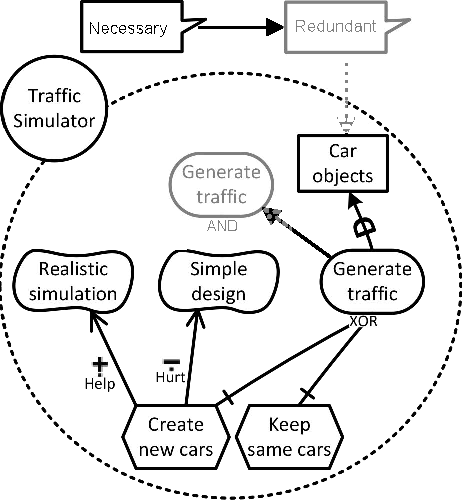
\includegraphics[width=\columnwidth]{img/Example1-new-attack.pdf}
\caption{Example RationalGRL model (extension of Fig.~\ref{fig:example-small2})}
\label{fig:example-small3}
\end{figure} 

We illustrate the new elements using Figure~\ref{fig:example-small3}, which is an extension of Figure~\ref{fig:example-small2}. 

We start with the new element which we call the \emph{Generic Argument}.

\begin{definition}[Generic Argument]
\label{def:generic-argument}
A generic argument $ga \in \mathbb{N}\times \{GenArg\}\times Names$ is a tuple such that $ga=(id, GenArg, name)$ means
\begin{itemize}
\item $id\in \mathbb{N}$ is the identifier of the generic argument,
\item $GenArg$ states that the tuple is a generic argument,
\item $name\in Names$ is a string description of its name.
\end{itemize}
We may refer to the argument with id $i$ simply with $ga_i$. A set of arguments is denoted by $GA$.
\end{definition}

\paragraph{Rationale and example} A generic counterargument is simply an argument that can be used to attack any previous argument, or an IE. Note that one of the constraints of a GRL model (Def.~\ref{def:grl-model}) is that GRL links (Def.~\ref{def:link}) should connect IEs, which means that in GRL generic arguments cannot be connected with GRL links. This is desired, since generic arguments are not part of GRL, so they should also not be connected using GRL links. 

In Fig.~\ref{fig:example-small3}, there are two generic counterargument which can be formalized as $(18,GenArg, \text{Redundant})$ and $(19, GenArg, \text{Necessary})$.

\begin{definition}[Argument]
\label{def:argument}
An argument $A$ is on of the following tuples:
\begin{itemize}
\item An intentional element (Def.~\ref{def:ie}), 
\item An actor $act$ (Def.~\ref{def:actor}),
\item An Actor-IE relation $r_{ActIE}$ (Def.~\ref{def:act-ie-relation}), 
\item A link $link$ (Def.~\ref{def:link}),
\item A generic argument $ga$ (Def.~\ref{def:generic-argument}).
\end{itemize}
\end{definition}

\paragraph{Rationale and example} We define an argument as either a generic argument or any of the GRL elements or links. This captures the specification in the RationalGRL metamodel (Fig.~\ref{fig:metamodel}) in which the class \textsf{Argument} is a superclass of \textsf{GenericArgument} and \textsf{GRLModelElement}, which again is a superclass of both \textsf{ElementLink} and \textsf{GRLLinkableElement}. A \textsf{GRLLinkableElement} is in turn a superclass of \textsf{Actor} and \textsf{IntentionalElement}. In sum, we define an argument simply as any one of the GRL elements or links, or a generic argument.

In Fig.~\ref{fig:example-small3}, the actor, all IEs, all links, and all generic counterarguments are arguments. We will give a full formalization of this after the definition of a RationalGRL model (Def.~\ref{def:rationalgrl-model}).

\begin{definition}[Attack Link]
\label{def:link:attack}
Given a set of arguments $Arg$, an attack link $att\in Arg\times Arg$ is a relation such that $att=(A_i,A_j)$ means:
\begin{itemize}
\item $A_i\in Arg$ is the argument performing that attack,
\item $A_j\in Arg$ is the argument being attacked.
\end{itemize}
Intuitively, $att=(A_i,A_j)$ means that argument $A_i$ is attacking argument $A_j$. A set of attack links is denoted by $Att$.
\end{definition}

\paragraph{Rationale and example} The attack link is the only link that RationalGRL adds to GRL. In Fig~\ref{fig:example-small3}, there are three attack links. The first two attack links originate from generic counterarguments and involve the following three arguments:
\begin{itemize}
\item $A_1 = (1, Resource, \text{Car objects}, AND)$
\item $A_{18} = (18, GenArg, \text{Redundant})$
\item $A_{19} = (19, GenArg, \text{Necessary})$
\end{itemize}

These two attack links are formalized as $(A_{18},A_{1})$ and $(A_{19}, A_{18})$.

The third attack link is an attack link created by \emph{replacing} and existing argument (we will discuss this process in more detail in Sect.~\ref{sect:algorithms}). It involves two version of the same IE:
\begin{itemize}
\item $A_{4} = ((4, Goal, \text{Generate traffic}, AND), Goal)$
\item $A_{20} = ((4, Goal, \text{Generate traffic}, XOR), Goal)$
\end{itemize}

This attack link is formalized at $(A_{20},A_4)$.

The last example shows an important difference between RationalGRL models and valid GRL models: While a valid GRL model disallows multiple elements with the same identifier (Def.~\ref{def:valid-grl-model}, condition 1), RationalGRL models do not enforce this restriction. This is because it is possible to create multiple arguments for the same element, where argument contains different content for the same element. This is what the example above also shows. However, the set of \emph{accepted} elements in a RationalGRL should all have unique identifier (see Def.~\ref{def:valid-rationalgrl-model}).

\begin{definition}[RationalGRL Model]
\label{def:rationalgrl-model}
A \emph{RationalGRL model} $RatGRL=(Arg, Att)$ consists of a set of arguments $Args$ (Def.~\ref{def:argument}) and a set of attack links $Att$ (Def.~\ref{def:link:attack}).
\end{definition}

\paragraph{Rationale and example} The definition of a RationalGRL model collects all the previously defined tuples into a single definition. For completeness, we now provide the full specification of Figure~\ref{fig:example-small3}. Let us first enumerate all the arguments used in this example:
\begin{flalign*}
A_0 = &(0, Actor, \text{Traffic simulator})&\\
A_1 = &(1, Task, \text{Car objects}, AND),&\\
A_2 = &(2, Softgoal, \text{Real. sim.}, AND),&\\
A_3 = &(3, Softgoal, \text{Simple des.}, AND),&\\
A_4 = &(4, Goal, \text{Generate traffic}, AND),&\\
A_5 = &(5, Task, \text{Create new cars}, AND),&\\
A_6 = &(6, Task, \text{Keep same cars}, AND),&\\
A_7 = &(7, Dep, 4, 1),&\\
A_8 = &(8, PosContr, 5, 2),&\\
A_9 = &(9, NegContr, 5, 3),&\\
A_{10} = &(10, Decomp, 5, 4),&\\
A_{11} = &(11, Decomp, 6, 4),&\\
A_i = &(i, ActIE, 0,i+11),ActIE), \text{for } 1\le i\le 6&\\
A_{18} = &(18, GenArg, \text{Redundant}),&\\
A_{19} = &(19, GenArg, \text{Necessary}),&\\
A_{20} = &(4, Goal, \text{Generate traffic}, XOR),&\\
\end{flalign*}

This model is then formalized as $RationalGRL=(Arg, Att)$ where:
\begin{flalign*}
Arg = &\{A_0,A_1,\ldots,A_{20}\}\\
Att=&\{(A_{18},A_1), (A_{19},A_{18}), (A_{20},A_{4})\}
\end{flalign*}

All the arguments and the attack relations of this RationalGRL model are shown in Figure~\ref{fig:example-small4}. Note the arguments for Actor-IE containment (arguments $A_{12}$ to $A_{17}$) have been omitted from this figure for readability. It can be read from the figure that two arguments are currently rejected, namely $A_4$ and $A_{19}$. However, we did not yet make precise how exactly this is computed. We will do so in the following definitions.

\begin{figure}[ht]
\centering
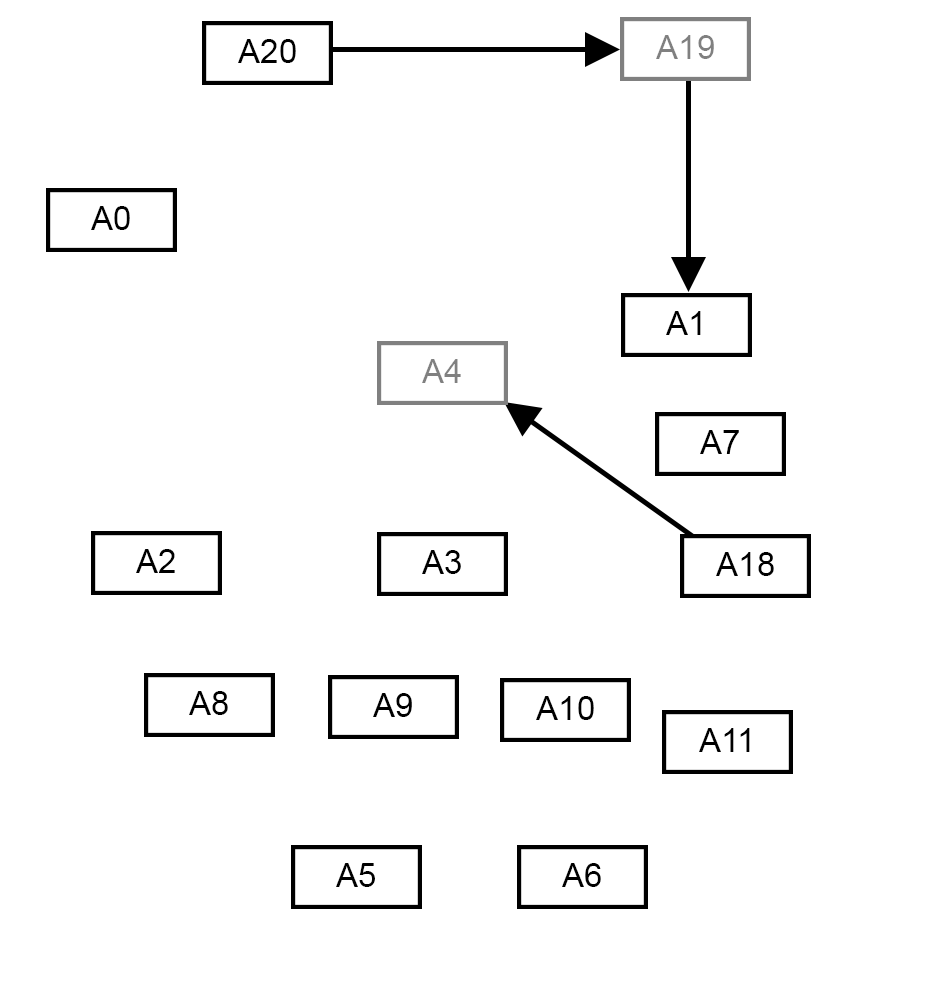
\includegraphics[width=\columnwidth]{img/Example1-new-arguments}
\caption{Argumentation framework of RationalGRL model from Fig.~\ref{fig:example-small3}}
\label{fig:example-small4}
\end{figure} 


In order to compute when an argument is accepted and when not we use argumentation semantics.  We use the standard approach here, which is known as \emph{Dung's semantics}. The following notions are preliminary.

\begin{definition}[Argumentation Framework~\cite{Dung1995}]
\label{def:argumentation-framework}
An \emph{argumentation framework} $AF=(Arg,Att)$ consists of a set of arguments $Arg$ and a set of attack relations $Att\subseteq Arg\times Arg.$
\end{definition}

We see that the definition of an argumentation framework is very close to that of a RationalGRL model. This allows us to use the following results directly.

\begin{definition}[Attack, conflict-freeness, defense, and admissibility~\cite{Dung1995}] Suppose an argumentation framework $AF=(Arg,Att)$, two sets of arguments $S\cup S'\subseteq Arg$, and some argument $A\in Arg$. We say that
\begin{itemize}
\item $S$ \emph{attacks} $A$ if some argument in $S$ attacks $A$,
\item $S$ \emph{attacks} $S'$ if some argument in $S$ attacks some argument in $S'$,
\item $S$ is \emph{conflict-free} if it does not attack itself,
\item $S$ \emph{defends} $A$ if for each $B$ such that $B$ attacks $A$, $S$ attacks $B$,
\item $S$ is \emph{admissible} if $S$ is conflict-free and defends each argument in it.
\end{itemize}
\end{definition}

\begin{figure}[ht!]
\centering
\begin{tikzpicture}
        \node[minimum size=1cm] (a19) [argNodeIN] at (-3,0) {$A_{19}$};
        \node[minimum size=1cm] (a18) [argNodeIN] at (0,0) {$A_{18}$};
        \node[minimum size=1cm] (a1) [argNodeIN] at (3,0) {$A_1$};
             
         \path
    (a19) edge [attackLink] (a18)
    (a18) edge [attackLink] (a1);
    
\end{tikzpicture}
\caption{Example argumentation framework, subset of Fig.~\ref{fig:example-small4}.}
\label{fig:goalmodeling:arg2}
\end{figure}

Let us explain these definitions using the example argumentation framework in Figure~\ref{fig:goalmodeling:arg2}, which is a subset of Figure~\ref{fig:example-small4} containing only arguments $A_1, A_{18}$, and $A_{19}$. In this example, there are two admissible sets: $\{A_{19}\}$ and $\{A_1, A_{19}\}$. In the last admissible set, $A_{19}$ defends $A_1$ against its attacker $A_{18}$. Sets containing both $A_{18}$ and either $A_1$ or $A_{19}$ are not conflict free, and the sets $\{A_1\}$ and $\{A_{18}\}$ do not defend themselves against $A_{18}$ and $A_{19}$, respectively. 

Given the notion of admissible sets, we can then define our argumentation semantics. There are a large number of different semantics to determine which arguments are acceptable; in this article, we focused on the preferred semantics.

\begin{definition}[Preferred semantics~\cite{Dung1995}] 
\label{def:preferred-semantics}
A preferred extension of an argumentation framework $(Arg,Att)$ is a maximal (w.r.t. set inclusion) admissible set of $R$.
\end{definition}

In our example from Figure~\ref{fig:goalmodeling:arg2}, there is one preferred extension, namely $\{A_{19},A_1\}$. Returning to our running example of Figure~\ref{fig:example-small3}, this means that the intentional elements \text{Car objects} (task) and the generic counerargument \emph{Necessary} are both \emph{accepted}, while the generic counter argument ``Redundant'' is rejected.

Now that we have defined the semantics for RationalGRL, we can use this to define the notion of a valid RationalGRL model.

\begin{definition}[Valid RationalGRL Model]
\label{def:valid-rationalgrl-model}
A RationalGRL model $RatGRL = (Arg, Att)$ with preferred extension $E=(A_1,\ldots,A_n)$ is a \emph{valid RationalGRL model} iff the GRL model constructed from $E$ is a valid GRL model (Def.~\ref{def:valid-grl-model}).
\end{definition}

\todo{Marc}{Marc}{Perhaps say something about how to construct it. It is very trivial: Just remove the generic arguments and attack links, only keep the other arguments which directly translate to GRL elements and links.}

\subsection{Algorithms for argument schemes and critical questions}
\label{sect:algorithms}

In the previous subsection we formalized a \emph{static} representation of the RationalGRL framework. In this section we formalize the \emph{dynamics}. We do so by developing algorithms for applying argument schemes and critical questions in the context of a RationalGRL model (Def.~\ref{def:rationalgrl-model}). These algorithms are applied to RationalGRL models and produce new arguments and attack relations. We can then use argumentation semantics (Def.~\ref{def:semantics}) to compute sets of accepted arguments. The content of these arguments is then used to compute the resulting RationalGRL model, together with enabled and disabled GRL elements and their underlying arguments.

As discussion in Section~\ref{sect:overview}, ll the argument schemes and critical questions of Table~\ref{table:argument-schemes} fall into one of the following four categories:
\begin{itemize}
\item \emph{INTRO}: These algorithms add one or multiple new arguments to the RationalGRL model, without creating any attack links. The arguments are for new GRL elements or links.
\item \emph{DISABLE}: These algorithms add a single argument to the RationalGRL model, which attacks one of multiple existing arguments. The counterargument that is added does not correspond to any GRL element, but instead disables an existing one by attacking all arguments for it.
\item \emph{REPLACE}: These algorithms can be seen as a combination of \emph{INTRO} and \emph{DISABLE}. They add a new argument corresponding to a GRL element or link, and this new argument attacks a previous version of the element or link. 
\end{itemize}

The three subsections of this section correspond to these three types of arguments.

In all of the following algorithms, we assume the following
\begin{itemize}
\item There algorithms are being applied to some valid RationalGRL model $RatGRL$ (Def.~\ref{def:valid-rationalgrl-model}),
\item The procedure $mindId()$ generates a new unique id.
\end{itemize}

\subsubsection{INTRO algorithms}

The following arguments schemes and critical questions of Table~\ref{table:argument-schemes} fall into this category:
\begin{itemize}
\item AS0-AS12
\item CQ5b, CQ6b, CQ6c, CQ7b, CQ9, CQ10b
\end{itemize}

These type of algorithms are short, and consist simply of adding an argument for the element that is being added. Since the structure of these algorithms are all very similar, we do not discuss them all. 

\begin{algorithm}[h]
  \caption{AS0: $a$ is an actor}\label{alg:add-actor}
  \begin{algorithmic}[1]
    \Procedure{$AS_0$}{$n$}
    \State $A \leftarrow (mintId(), Actor, a)$ \label{alg:as0:1}
    \State $Arg\leftarrow Arg \cup \{A\}$\label{alg:as0:2}
    \EndProcedure
  \end{algorithmic}
\end{algorithm}

\paragraph{Rationale and example} Algorithm takes one argument, namely the name of the actor $a$. On line~\ref{alg:as0:1} of the algorithm, a new (unique) id is minted as the identifier of the new actor, which is assigned with its corresponding name to the variable $actor$. On line~\ref{alg:as0:2} the actor is added as a new argument.

Consider for instance...\todo{Marc}{Marc}{Add example}

\begin{algorithm}[h]
  \caption{AS1: Actor with id $i$ has resource $R$}\label{alg:add-actor}
  \begin{algorithmic}[1]
    \Procedure{$AS_1$}{$i, R$}
    \State $res\_id\gets mintId()$\label{alg:add-actor:id}
    \State $A_1\leftarrow (res\_id, Resource, R, AND)$\label{alg:add-actor:arg1}
    \State $A_2\leftarrow (mintId(),ActIE, i, res\_id)$\label{alg:add-actor:arg2}
    \State $Arg\gets Arg\cup \{A_1,A_2\}$\label{alg:add-actor:add-arg}
    \EndProcedure
  \end{algorithmic}
\end{algorithm}

\paragraph{Rationale and example} The original argument schemes AS1 is phrased as ``Actor $a$ has resource $R$''. We have slightly reworded this in Algorithm~\ref{alg:add-actor} to ``Actor with id $i$ has resource $R$''. The reason is that in GRL, actors have identifiers, so since we assume actor $a$ exists already, we also assume an identifier for it exists. It would be straightforward to introduce a mapping from actor names to identifiers, but we have no done so here for simplicity. 

The algorithm itself runs as follows: on line~\ref{alg:add-actor:id}, a unique id is assigned to variable $res\_id$ (``resource identifier''). On line~\ref{alg:add-actor:arg1}, an argument for a resource with name $R$ and identifier $res\_id$ is assigned to $A_1$. On line~\ref{alg:add-actor:arg2}, a second argument $A_2$ is created, which is an argument for an Actor-IE relation (Def.~\ref{def:act-ie-relation}) between the input actor $i$ and the newly created element $res\_id$. Finally, on line~\ref{alg:add-actor:add-arg}, the arguments are added to the set of arguments $Arg$.

Since arguments schemes AS2-AS4 are very similar to AS1, we have omitted algorithms for them here.

\begin{algorithm}[h]
  \caption{AS5: Goal with id $i$ decomposes into task $T$}\label{alg:add-decomp}
  \begin{algorithmic}[1]
    \Procedure{$AS_5$}{$i, T$}
    \State $task\_id\gets mintId()$\label{alg:add-decomp:task-id}
    \State $A_1\leftarrow (task\_id, Task, t, AND)$\label{alg:add-decomp:arg1}
    \State $A_2\leftarrow (mintId(), Decomp, i, task\_id)$\label{alg:add-decomp:arg2}
    \State $Arg\gets Arg\cup \{A_1,A_2\}$\label{alg:add-decomp:add-arg}
    \EndProcedure
  \end{algorithmic}
\end{algorithm}

\paragraph{Rationale and example} Similar to the previous algorithm, we have slightly reworded critical question AS5. We assume that a goal $G$ exists already with identifier $i$, and that some new task with name $T$ is a decomposition of $G$. 

In Algorithm~\ref{alg:add-decomp}, on line~\ref{alg:add-decomp:task-id} a unique identifier is created for the task, which is created on line~\ref{alg:add-decomp:arg1}. On line~\ref{alg:add-decomp:arg2} an argument is created for the decomposition link $(mintId(), Decomp, i, task\_id)$ (Def.~\ref{def:link}, going from the existing goal with identifier $i$ to the new task with identifier $task\_id$. On line~\ref{alg:add-decomp:add-arg} the two arguments are added to the set of arguments $Arg$.

The remaining argument schemes AS6-AS12 are all very similar to the previous algorithms and have been omitted here.

The critical questions of type \emph{INTRO} are very similar as well, with one exception: the require an answer. For instance, suppose CQ5b: ``Does goal $G$ decompose into other tasks?'' is answered with: ``Yes, namely into task $T$''. In this case, we simply obtain an instantiation of argument scheme AS5: ``Goal $G$ decomposes into task $T$'', which can be executed with Algorithm~\ref{alg:add-decomp}. This is the same for all the other critical questions of type \emph{INTRO} as well. Therefore, we have omitted them here as well.

\subsubsection{DISABLE algorithms}

As discussed before, algorithms of type \emph{DISABLE} consist of adding a new argument attacking an existing argument, which is an argument for an existing GRL element or link. The argument that is added is itself not an argument for a GRL element or link.

In all of these algorithms, we assume the critical question is answered affirmatively. For instance, for critical question CQ0 ``Is the actor relevant?'', we assume it is answered with ``No'' (see right-most column of Table~\ref{table:argument-schemes}).

\begin{algorithm}[h]
  \caption{CQ0: Is actor with id $i$ relevant? No}\label{alg:actor-not-relevant}
  \begin{algorithmic}[1]
    \Procedure{$CQ_0$}{$i$}
    \State $A \leftarrow (mintId(),GenArg,CQ0)$\label{alg:actor-not-relevant:genarg}
    \State $Arg\leftarrow Arg \cup \{A\}$\label{alg:actor-not-relevant:genarg2}
    \For{$A_j\in \{A=(i,Actor,n)\mid A\in Arg\}$}\label{alg:actor-not-relevant:for}
      \State $Att \leftarrow Att \cup \{(A,A_j)\}$\label{alg:actor-not-relevant:att}
    \EndFor
    \EndProcedure
  \end{algorithmic}
\end{algorithm}

\paragraph{Rationale and example} Algorithm~\ref{alg:actor-not-relevant} is executed when critical question CQ0 is answered affirmatively (i.e., with ``No''). First, on lines~\ref{alg:actor-not-relevant:genarg} and~\ref{alg:actor-not-relevant:genarg2}, an argument is created for the critical question and added to the set of arguments $Arg$. Since this argument is not an argument for a GRL element or link, it is formalized as a \emph{generic counterargument} $(mintId(), GenArg, CQ0)$ (Def.~\ref{def:generic-argument}). The for loop starting at line~\ref{alg:actor-not-relevant:for} then iterates over all arguments for actors, where $i$ is the id of the actor that is no longer relevant. The reason why there could be multiple of such actors is that the actor can be refined by an algorithm of type \emph{REPLACE}. We will explain this in more detail in the example below. Then, on line~\ref{alg:actor-not-relevant:att}, an attack link is created from the generic argument $A$ that is created to the argument for the actor $A_j$. After executing the algorithm, all existing arguments for the actor with identifier $i$ are attacked by a newly created argument $A$.

Consider for example...\todo{Marc}{Marc}{Add example here}

Critical questions C1-CQ3 are all very similar to CQ0 and have therefore been omitted here.

\begin{algorithm}[h]
  \caption{CQ5a: Does the goal with id $g\_id$ decompose into task with id $t\_id$? No}\label{alg:no-decomp}
  \begin{algorithmic}[1]
    \Procedure{$CQ5a$}{$g\_id,t\_id$}
    \State $A \leftarrow (mintId(),GenArg,CQ5a)$\label{alg:no-decomp:genarg}
    \State $Arg\leftarrow Arg \cup \{A\}$\label{alg:no-decomp:genarg2}
    \For{$A_j\in \{(k,Decomp,g\_id,t\_id)\in Arg\}$}\label{alg:no-decomp:for}
      \State $Att \leftarrow Att \cup \{(A,A_j)\}$\label{alg:no-decomp:att}
    \EndFor
    \EndProcedure
  \end{algorithmic}
\end{algorithm}

\paragraph{Rationale and example} Algorithm~\ref{alg:no-decomp} is structurally very similar to Algorithm~\ref{alg:actor-not-relevant}, with the only difference that instead of iterating over actors, we now iterate over decomposition links. This is done in line~\ref{alg:no-decomp:for}, where we iterate over all decomposition links with source id $g\_id$ and target id $t\_id$ (Def.~\ref{def:link}). This means we iterate over all decomposition links from the goal to the task, and we attack all arguments for these links on line~\ref{alg:no-decomp:att} with the newly created argument.

Almost all of the remaining critical questions of type DISABLE are similar in structure. CQ11 (``Is the element relevant/useful'') is slightly different since the attack element is not of a specific type, but is simply any GRL element. However, the resulting algorithm is very similar to the previous two and has therefore been omitted. The only algorithm of type \emph{DISABLE} that we still discuss is $Att$.

\begin{algorithm}[h]
  \caption{Att: Generic counter-argument on arguments $A_1,\ldots,A_n$ with name $N$}\label{alg:generic}
  \begin{algorithmic}[1]
    \Procedure{$Att$}{$A_1,\ldots,A_n$, $N$}
    \State $A \leftarrow (mintId(),GenArg, N)$\label{alg:generic:arg}
    \State $Arg\leftarrow Arg \cup \{A\}$\label{alg:generic:addarg}
    \For{$A_j\in \{A_1,\ldots,A_n\}$}\label{alg:generic:for}
      \State $Att \leftarrow Att \cup \{(A,A_j)\}$\label{alg:generic:att}
    \EndFor
    \EndProcedure
  \end{algorithmic}
\end{algorithm}

\paragraph{Rationale and example} Algorithm~\ref{alg:generic} can be regarded as the most general way of providing counter-arguments to arguments. In all of the previous \emph{DISABLE} algorithm, the attack was on a specific type of argument, for instance an argument for an actor or an argument for a decomposition. In this algorithm, however, \emph{any} set of arguments can be attacked by a new argument.

\todo{Marc}{Marc}{Give example}

\subsubsection{REPLACE algorithms}

Recall that the \emph{REPLACE} algorithms both attacks all arguments for an existing element, and at the same time create a new argument that contains a different version of the element being attacked.

\begin{algorithm}[h]
  \caption{CQ5c: Is the decomposition type of element $ie_i$ correct? No, it should be $X$ }\label{alg:replace1}
  \begin{algorithmic}[1]
    \Procedure{$CQ5c$}{$ie_i, X$}
    \State $A \leftarrow ie_i$\label{alg:replace1:arg}
    \State $A.decomptype\leftarrow X$\label{alg:replace1:decompchange}
    \State $IEArgs\leftarrow IE_i\subseteq  Arg$\label{alg:replace1:ieargs}
    \For{$A_i\in IEArgs$}\label{alg:replace1:for1}
      \State $Att \leftarrow Att \cup \{(A,A_i)\}$\label{alg:replace1:att}
    \EndFor
    \For{$\{(A_i,A_j)\in Att\mid A_j\in IEArgs\}$}\label{alg:replace1:for2}
      \State $Att\leftarrow (A_i,A)$
    \EndFor
    \For{$\{(A_i,A_j)\in Att\mid A_i\in IEArgs\}$}\label{alg:replace1:for3}
      \State $Att\leftarrow (A,A_j)$
    \EndFor
    \State $Arg\leftarrow Arg \cup \{A\}$\label{alg:replace1:addarg}
    \EndProcedure
  \end{algorithmic}
\end{algorithm}

\paragraph{Rationale and example} While the original critical question CQ5c is specific to the decomposition between a goal and a task, Algorithm~\ref{alg:replace1} is more generally applicable to any IE, since all IEs have a decomposition type in their definition (Def.~\ref{def:ie}). 

Let us go through this algorithm step by step. On line~\ref{alg:replace1:arg}, a new argument $A$ is created which is identical to original IE. Recall from Def.~\ref{def:notation} that we may refer to elements of an IE with the ``.'' notation. This is what we do on line~\ref{alg:replace1:decompchange}, where the decomposition type of the argument is changed to $X$. On line~\ref{alg:replace1:ieargs}, the set $IEArgs$ is assigned with all existing arguments for the input IE (recall the notation of $IE_i$ as the set of all IEs with id $i$, see Def.~\ref{def:notation}). Then, in the first for loop on line~\ref{alg:replace1:for1}, we add attack links from the argument that has just been created to all existing arguments for the IE. The next two for loops on respectively lines~\ref{alg:replace1:for2} and~\ref{alg:replace1:for3} ensure that all attack links that existing from and to the previous versions of the IE are also carried over to the new argument $A$. Finally, one line~\ref{alg:replace1:addarg}, the new argument is added to the set of arguments.

Let us explain this with an example. \todo{Marc}{Marc}{Add example}

The other \emph{REPLACE} algorithms are very similar to Algorithm~\ref{alg:replace1}. It can be used directly for CQ10c, but for CQ12 we should make a small modification. Instead of replacing the decomposition type of the IE, we should replace its name. Since this is a very minor modification we have omitted it here.
